\documentclass{article}
\usepackage{algorithm2e}
\usepackage{graphicx}
\title{CME211 Final Project Part 1}
\author{Prarthna Khemka}

\begin{document}
\maketitle

\section{Overview}
This project involves creating a program to solve the 2D steady state heat
equation on a simple geometry using a sparse matrix solver and finite
difference and Conjugate Gradient Methods. The system to be solved is one
where hot liquid is being transferred in the pipe which is being cooled with
cool air jets. The goal is to find the mean temperature within pipe walls
which is done through analysis of a periodic section of the pipe wall. 

\section{Program Implementation}
Three main elements of the program:
\begin{itemize}
\item The CG algorithm:
  Solves the linear system Ax = b with A sparse where A would reflect
  the heat system being analyzed in this case. x is used as u in the
  pseudocode for efficient storage. b is the solution vector. The CG
  algorithm uses only 4 helper functions for efficient coding. 
\item Sparse Matrix:
  A class that contains the structure of sparse matrix A. It has methods
  to resize the matrix in the required form, add entries in the matrix,
  convert to CSR storage efficiency, and ability to perform matrix vector
  multiplication. We use this sparse matrix A in the HeatEquation2D class.
\item HeatEquation2D:
  A class that sets up the system where A is filled in based on the pipe
  stencil, x as an initial guess of 1s, and b as temperatures based on the
  point in the pipe stencil. These 3 attributes are then passed to the
  solver which invokes the CGSolver and writes the solution to output files.
\end{itemize}
Here is the pseudocode for the CG Algorithm:

\begin{algorithm}[H]
  \caption{CG Algorithm}
  \SetAlgoLined
  Initialize {$x_0$}\;
  $r_0 = b - Ax_0$\;
  $L2normr0 = ||r_0||_2$\;
  $p_0 = r_0$\;
  $niter = 0$\;
  \While{$niter < nitermax$}{
    $niter = niter + 1$\;
    $alpha = ({r_n}^T r_n) / ({p_n}^T  A  p_n)$\;
    $x_{n+1} = x_n + alpha  p_n$\;
    $r_{n+1} = r_n - alpha  A  p_n$\;
    $L2normr = ||r_{n+1}||_2$\;
    \If{$L2normr/L2normr0 < threshold$}{
      break\;
    }
    $beta = (r_{n+1}^T  r_{n+1}) / ({r_n}^T  r_n)$\;
    $p_{n+1} = r_{n+1} + beta  p_n$\;
  }
  
\end{algorithm}

\section{Users Guide}
System Solved in C++:
To compile the code, use the make command which is provided by the makefile.
To run the program from the command line call main with input file and
solution prefix. Running this will result in an output that alerts if the
solver converges or not in the solver and creates solutions files.

Postprocessing and visualization in Python:
The python file computes the mean temperature and creates pseudocolor plots
for temperature distribution in the pipe.
To run the program from the command line call python3 with postprocess.py
input file and solution file. 

\section{Visualization from post processing}
\begin{figure}
  \centering
  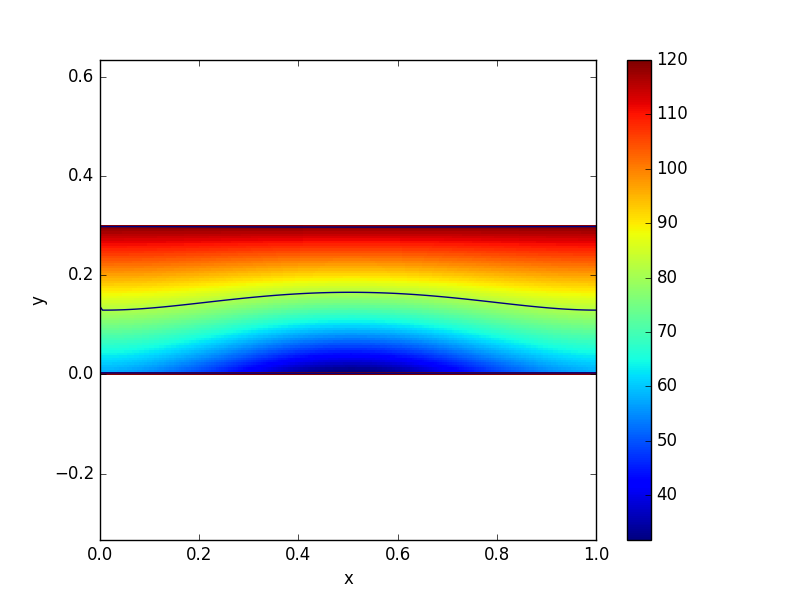
\includegraphics[width = 15cm, height = 12cm]{plot.png}
  \caption{Pseudocolor plot for input2.txt solution}
\end{figure}

\pagebreak

\begin{thebibliography}{5}
\bibitem{item1} cme211-project-part-1.pdf
\bibitem{item2} cme211-project-part-2.pdf
\end{thebibliography}
  
\end{document}
  
